\documentclass[tikz,border=3pt]{standalone}
\usepackage[utf8]{inputenc}
\usepackage[T1]{fontenc}
\usepackage{lmodern}
\renewcommand{\familydefault}{\sfdefault}
\usepackage{sansmath}\sansmath
\usepackage{chemfig}
\usepackage{pgfplots}\pgfplotsset{compat=1.18,/pgf/number format/use comma,/pgf/number format/1000 sep={.}}
\usetikzlibrary{arrows.meta,calc,positioning,decorations.pathmorphing,patterns}
% paleta del sitio
\definecolor{nar}{HTML}{E8680C}\definecolor{narc}{HTML}{FFB35C}\definecolor{hielo}{HTML}{FFF3E8}
\definecolor{tinta}{HTML}{1D1D1F}\definecolor{gris}{HTML}{6E6E73}\definecolor{lila}{HTML}{7C5CF0}
\definecolor{azul}{HTML}{2F6FD6}\definecolor{menta}{HTML}{17A673}\definecolor{coral}{HTML}{E8342A}
\begin{document}
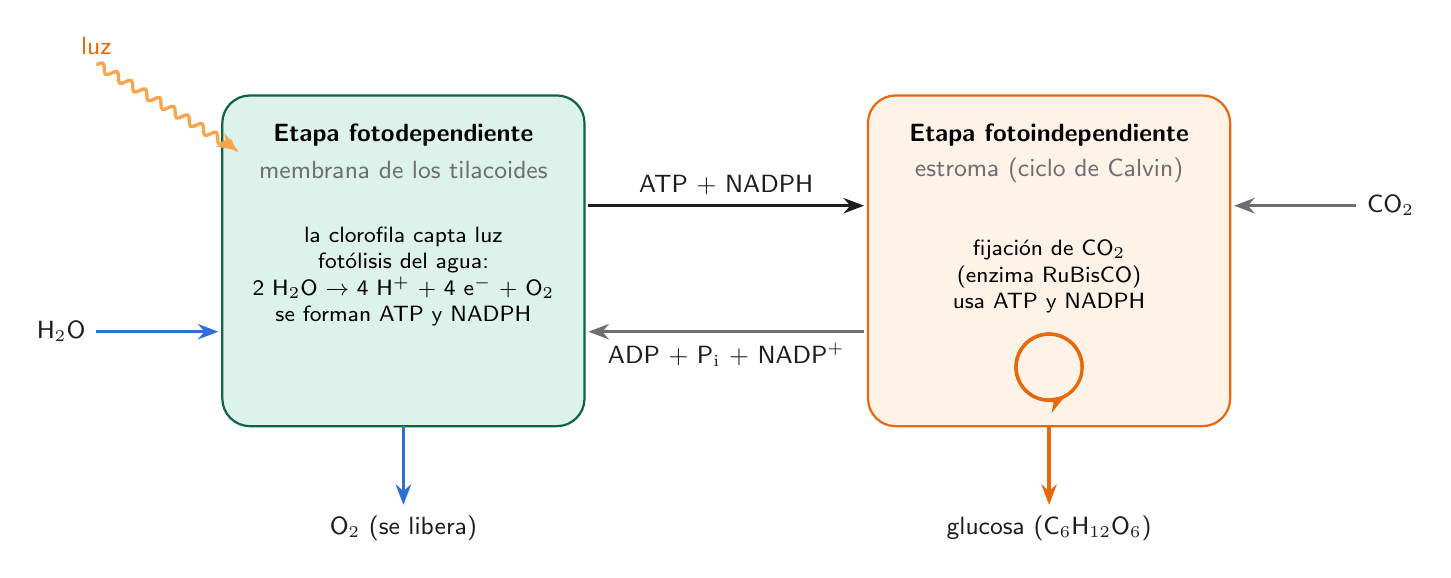
\begin{tikzpicture}[font=\small,>={Stealth[length=2.6mm]}]
\draw[menta!60!black,thick,fill=menta!15,rounded corners=10pt] (0,0) rectangle (4.6,4.2);
\draw[nar,thick,fill=hielo,rounded corners=10pt] (8.2,0) rectangle (12.8,4.2);
\node[font=\small\bfseries,align=center] at (2.3,3.7) {Etapa fotodependiente};
\node[text=gris,align=center] at (2.3,3.25) {membrana de los tilacoides};
\node[font=\small\bfseries,align=center] at (10.5,3.7) {Etapa fotoindependiente};
\node[text=gris,align=center] at (10.5,3.25) {estroma (ciclo de Calvin)};
\node[align=center,font=\footnotesize] at (2.3,1.9) {la clorofila capta luz\\fotólisis del agua:\\2 H$_2$O $\to$ 4 H$^+$ + 4 e$^-$ + O$_2$\\se forman ATP y NADPH};
\node[align=center,font=\footnotesize] at (10.5,1.9) {fijación de CO$_2$\\(enzima RuBisCO)\\usa ATP y NADPH};
\draw[nar,very thick] (10.5,0.75) circle (0.42);
\draw[nar,very thick,->] (10.92,0.75) arc (0:300:0.42);
% luz
\draw[narc!80!nar,very thick,decorate,decoration={snake,amplitude=1.5pt,segment length=6pt},->] (-1.6,4.6) -- (0.2,3.5);
\node[anchor=south,text=nar] at (-1.6,4.6) {luz};
\draw[azul,very thick,->] (-1.6,1.2) -- (-0.05,1.2) node[pos=0,anchor=east,text=tinta] {H$_2$O};
\draw[azul,very thick,->] (2.3,0) -- (2.3,-1.0) node[anchor=north,text=tinta] {O$_2$ (se libera)};
\draw[tinta,very thick,->] (4.65,2.8) -- (8.15,2.8) node[midway,above] {ATP + NADPH};
\draw[gris,very thick,->] (8.15,1.2) -- (4.65,1.2) node[midway,below,text=tinta] {ADP + P$_\mathrm{i}$ + NADP$^+$};
\draw[gris,very thick,->] (14.4,2.8) -- (12.85,2.8) node[pos=0,anchor=west,text=tinta] {CO$_2$};
\draw[nar,very thick,->] (10.5,0) -- (10.5,-1.0) node[anchor=north,text=tinta] {glucosa (C$_6$H$_{12}$O$_6$)};
\end{tikzpicture}
\end{document}
